
\documentclass[runningheads,a4paper]{llncs}

\usepackage[utf8]{inputenc}            % kodowanie
\usepackage[OT4]{fontenc}              % font PL
\usepackage[polish]{babel}
% \usepackage{amssymb}
\setcounter{tocdepth}{3}
\usepackage{graphicx}
\usepackage{epstopdf}
\usepackage{caption}
\captionsetup{compatibility=false}
\captionsetup{justification=centering}
\usepackage{subcaption}

\usepackage{url}
\urldef{\mailsa}\path|{alfred.hofmann, ursula.barth, ingrid.haas, frank.holzwarth,|
\urldef{\mailsb}\path|anna.kramer, leonie.kunz, christine.reiss, nicole.sator,|
\urldef{\mailsc}\path|erika.siebert-cole, peter.strasser, lncs}@springer.com|
\newcommand{\keywords}[1]{\par\addvspace\baselineskip
\noindent\keywordname\enspace\ignorespaces#1}

\renewcommand{\keywordname}{\textbf{Słowa kluczowe:}}

\setlength{\fboxsep}{0pt}
\setlength{\fboxrule}{1pt}

\begin{document}

\mainmatter
\title{Wykrywanie ataków w sieciach komputerowych z wykorzystaniem systemów Honeypot}
\author{Maciej Jagiełło}

\titlerunning{ }
\authorrunning{ }
\institute{}
\maketitle

\begin{abstract}
A tu będzie streszczenie!!!!!!!!!!!!!!!!!!!!!!!!!!!!!!1
\keywords{honeypot, glastopf, kippo, dionaea, vagrant, puppet, virtualbox}
\end{abstract}


\section{Wprowadzenie}

Wykrywanie ataków w sieciach komputerowych to ważny element działań na rzecz zwiększania bezpieczeństwa systemów. Cyberprzestępczość rozwija się szybkim tempem, z każdym dniem opracowywane są nowe sposoby ataków, wykorzystywane są nowe podatności w aplikacjach, protokołach i systemach operacyjnych. Aby temu przeciwdziałać, konieczne jest opracowanie odpowiednich narzędzi. ....

Celem systemu jest stworzenie narzędzia do zbierania adresów IP hakerów, botów i zainfekowanych maszyn w spójną bazę danych, którą będzie można później wykorzystać np. do rozszerzania reguł zapór ogniowych. System ma również utrwalać Ma być też źródłem nowych wirusów do analizowania przez antywirusy. Wybrane rozwiązanie problemu to sieć Honeypotów.

Honeypot to jedynie idea zbierania informacji. Jest to kombinacja ustawień sprzętowych i programowych, które tworzą system pułapkę. Ustawienia sprzętowe, czyli komputer, wyodrębniony obszar sieci lokalnej, który odpowiednio symuluje prawdziwą sieć, ale jest od niej odizolowany i zabezpieczony.

Taki system, uruchomiony na maszynie serwerowej, udostępnia w Internecie jakiś zasób atrakcyjny dla atakującego. Może to być rekord w bazie danych, aplikacja lub cały system operacyjny. Używając odpowiednich mechanizmów do monitorowania zachowania, zbiera dane o sposobach wykonywania ataków.

Jego główną zaletą jest to, że korzystają z niego niemal wyłącznie użytkownicy, którzy chcą włamać się do sieci.

\section{Sieć honeypotów}

Na rysunku \ref{fig:architektura_fig} przedstawiony jest schemat architektury aplikacji. Każdy honeypot uruchomiony jest w maszynie wirtualnej. Maszyna ta posiada dostęp do Internetu i wystawia do niego, odpowiednie dla zainstalowanych honeypotów, zasoby. Moduł pobierania i analizy logów zbiera pozostawione przez honeypoty informacje o atakujących. Są to ślady wykonywanych akcji i pliki binarne ładowane na maszyny przez atakujących.

\begin{figure}
        \centering
        \fbox{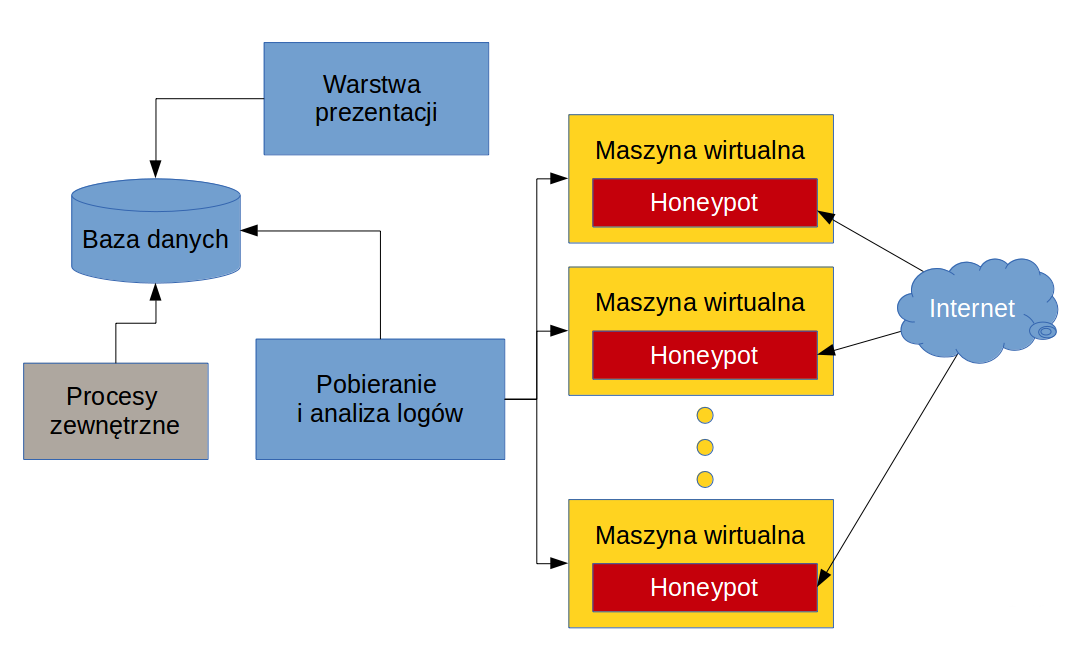
\includegraphics[width=1.0\textwidth]{pics/architektura}}
        \caption{Architektura aplikacji.}
        \label{fig:architektura_fig}
\end{figure}

Istnieje bardzo dużo realizacji honeypotów. Na stronie \cite{honeynet_project}, która zajmuje się rozwojem narzędzi do zwiększenia bezpieczeństwa w internecie, jest wymienione około 30 projektów, a to z pewnością nie wszystkie dostępne.

Warto wspomnieć o pracującym na wydziale Elektroniki i Technik Informacyjnych, doktorze Krzysztofie Cabaju, który na przedmiotach BSS, SKM2 i TKOM prowadzi studentów podczas implementacji jego autorskich honeypotów.

W opisywanym systemie zostały wybrane trzy realizacje honeypotów. Wybór ten  ze względu na wystarczającą różnorodność w oferowanych przez nie usługach.

\section{}

Szklany garnek. Pierwszy z prezentowanych honeypotów jest zwyczajną witryną www, którą można znaleźć w wyszukiwarkach internetowych.

Daje się znaleźć po frazach w języku angielskim, które są generowane z predefiniowanej bazy danych

Potrafi analizować zapytania HTTP, w szczególności zapytania GET, które w parametrze mają zdefiniowane ścieżki URL. Takie argumenty parsuje i próbuje ściągać na dysk do późniejszej analizy.
\section{}
Kolejnym wektorem ataków, na jaki są podatne komputery w sieciach komputerowych jest protokół ssh.

Kippo, poza oczywistymi dla mnie źródłem informacji o adresach IP, loguje całą sesję użytkownika od próby zalogowania do aktywności po wylogowaniu (po prostu przechwytuje „logout“, „exit“, SIGINT).

Po wylogowaniu wyświetla znak zachęty wyglądający jak na lokalnym komputerze.

Udostępnia fałszywy system plików, który wygląda jak po świeżej instalacji debiana. Nie da się tam nic zmienić, tylko niektóre polecenia działają tak jak prawdziwe (reszta zazwyczaj wyświetla komunikat o błędzie)

Tak jak poprzednik, Kippo pobiera i przechowuje pobrane przez atakującego pliki.
\section{}
Co tu dużo gadać, kolejny honeypot, tym razem z innymi protokołami. Działa
\section{}
Istotnym, choć niekoniecznym krokiem w stronę wewnętrznego bezpieczeństwa jest uruchamianie serwerów honeypotowych w maszynie wirtualnej.

Rozwiązanie bardzo przydatne gdy chcemy, by nasza maszyna była łatwo powielalna.

Vagrant natomiast jest świetnym narzędziem do automatyzacji stawiania takiej maszyny. Przygotowujemy kilka plików konfiguracyjnych w tym jeden z nich to skrypt instalacyjny na naszej maszynie.

Alternatywą do wirtualnej maszyny jest wirtualny kontener, który nie tworzy wirtualnego systemu od początku do końca, a tylko izoluje aplikację od systemu. Bez wchodzenia w szczegóły. Ten sposób jest o wiele lżejszy dla systemu, ale nie gwarantuje 100\% bezpieczeństwa.

Skrypt dostarczający aplikację może być napisany w Puppecie – narzędziu do deklaratywnego zarządzania stanem maszyny.
\section{}
Najprostsza wersja do użycia vagranta to trzy polecenia, około 5 minut czekania i jest postawiona maszyna wirtualna z ubuntu server w 32 bitowej wersji.

W moim systemie nie ma potrzeby logowania się do maszyny przez protokół ssh, jedyne co będzie potrzebne to uruchomienie vagrant up z odpowiednimi skryptami dostarczającymi instalację honeypota. W moim przypadku puppetowymi.

konsola
\section{}
Przykładowy i skrócony na potrzeby prezentacji plik puppetowy .

Kolejność, moduły, bashe (również warunki na OS), serwisy, paczki z pipa apt-geta niezależnie od systemu i bez promptów o hasło czy potwierdzenie kontynuacji

Wystarczy puppet apply

Możliwa architektura master-slave, ale nie używana w tym projekcie

\section{}
Aplikacja
Silnik zbierania danych napisany w Javie
Metadane o każdym honeypocie:
Lista lokalizacji plików do ściągnięcia
Reguły rozpoznawania plików tekstowych
Testy integracyjne z użyciem Vagranta, Virtualboxa i Puppeta
\section{}
Pierwszym problemem przy pobieraniu logów jest to, że ze względów bezpieczeństwa honeypot nie powinien mieć dostępu do żadnej części tworzonego systemu, ponieważ w przypadku włamania się na serwer, haker może zniszczyć nie tylko maszynę z honeypotem.

Najprostszym sposobem wyciągania logów jest użycie protokołu ssh. Nie wymaga instalowania dodatkowych aplikacji, wspiera przesyłanie plików, jest protokołem względnie bezpiecznym w porównaniu do innych autorskich rozwiązań.

Aby poradzić sobie z rosnącym w nieskończoność plikiem logów, trzeba go albo czyścić albo archiwizować.

\section{}
Dwa przykłady prezentacji na żywo ataków z sieci honeypotów.

Typy ataków, ip (lokacja), geoIP, live

To tylko warstwa prezentacji
\section{Podsumowanie}
Użyłem honeypotów ..., spełniły swoje zadanie. Pierwsze dane od botów skanujących internet pojawiły się już po paru dniach. Teraz jest to jakieś 500 ataków na godzinę.

Wdrażanie ich to proste uruchomienie skryptu.

Najczęściej spotyka się boty o nagłówkach HTTP, że to tylko zbieranie danych na potrzeby badań - „edukacyjne“

\section{}
\begin{thebibliography}{1}

% \bibitem{url} Xa,
% \url{http://xa}

\bibitem{} Ataki sieciowe,
\url{http://jbeczala.republika.pl/files/ataki_sieciowe.pdf}
\bibitem{honeynet_project} l, \url{https://www.honeynet.org/project}
\bibitem{} l,
\url{http://glastopf.org/}
\bibitem{} k,
\url{https://github.com/desaster/kippo}
\bibitem{} j,
\url{https://www.honeynet.org/project}
\bibitem{} h,
\url{http://map.ipviking.com/}
\bibitem{} g,
\url{http://digitalattackmap.com/}
\bibitem{} a,
\url{https://puppetlabs.com/}
\bibitem{} f,
\url{https://www.virtualbox.org/}
\bibitem{} 2w,
\url{https://www.vagrantup.com/}
\bibitem{} xa,
\url{http://www.digitalforreallife.com/2012/11/boosting-teamwork-with-vagrant/}


\end{thebibliography}

\end{document}
